\apendice{Documentación de usuario}

\section{Introducción}
En este último apéndice, se incluye la información necesaria para poder utilizar la aplicación del proyecto, como poder instalarlo y el manual de usuario para saber utilizar la aplicación.

\section{Requisitos de usuarios}
El primer requisito por parte del usuario es la necesidad de tener conexión a Internet, ya que los datos se encuentran alojados en una base de datos, por lo que para poder usarla será necesario tener conexión.

En segundo lugar, necesitará tener un entorno con todas las librerías que usa la aplicación, junto con alguna aplicación que permite ejecutar un \emph{notebook}, como, por ejemplo, \emph{Jupyter Notebook}.

Una vez se diponga de todo lo anterior, ya sería posible poder utilizar la aplicación que se ha llevado a cabo en este proyecto.

\section{Instalación}
En primer lugar, sería necesario descargar en instalar Anaconda en caso de que no se disponga de dicha herramienta. Ya que permite crear un entorno con todos los requisitos de la aplicación y se podrá usar sin ningún problema. Para ello, es tan sencillo como ir a la siguiente ruta:

\url{https://www.anaconda.com/download}

Y en ella descargar, la versión adecuada a tu sistema operativo. Tras esto, sería tan sencillo como seguir el instalador y esperar unos minutos a que termine la instalación.

En segundo lugar, habría que instalar las dependencias de la aplicación. Para facilitar este proceso se ha dejado en el repositorio del proyecto un fichero \emph{requirements}, obtenido de un entorno \emph{Windows}, que permitirá descargar todas las librerías junto con sus versiones que hacen que se garantice la posibilidad de utilizar la aplicación. Dicho fichero se puede encontrar en el siguiente enlace:

\url{https://github.com/ifh1001/TFM/blob/main/requirements.txt}

En tercer, y último lugar, para poder instalar las dependencias, se abrirá la consola \emph{Anaconda Prompt} y se escribirá el siguiente comando:

\begin{verbatim}
conda create --name nombre_entorno --file requirements.txt
\end{verbatim}

Y tras esperar unos minutos, se habrán instalado todas las dependencias, por lo que ya se ha creado un entorno que sea capaz de lanzar la aplicación.

\section{Manual del usuario}
En primer paso para poder utilizar la aplicación, es lanzar \emph{Jupyter Notebook}. Para ello, y basándose el apartado de instalación, lo primero sería cambiar al nuevo entorno, y posteriormente ejecutar el comando de la herramienta. Ambos comandos se muestran a continuación:

\begin{verbatim}
conda activate nombre_entorno

jupyter notebook
\end{verbatim}

Tras su ejecución aparecerá en el navegador la herramienta, y sería tan sencillo como dirigirse al directorio donde se encuentra el \emph{notebook} de la aplicación. Tras abrirlo se verá que hay 3 celdas y que habrá que ejecutar en orden. Para ejecutar una celda, hacemos clic sobre ella y pulsamos al botón \textbf{Run} que se encuentra en el menú superior, tras esperar un rato veremos como a la izquierda de la celda aparecerá un 1, de igual forma que se puede ver en la Figura \ref{f:celda1}.

\begin{figure}[h]
 \centering
  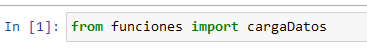
\includegraphics[width=0.7\textwidth]{img/celda1.PNG}
 \caption{Ejecución de la Primera Celda}
 \label{f:celda1}
\end{figure}

A continuación, será necesario ejecutar la segunda celda, o previamente modificar los valores en caso de que se quiera utilizar una base de datos diferente a la que viene por defecto. Tras su ejecución aparecerá a la izquierda un 2.

Finalmente, se ejecutará la última celda, y se verá como aparece un desplegable que muestra las IDs de todas las bobinas cargadas de la base de datos, Figura \ref{f:celda3}. Sería tan sencillo como seleccionar una y esperar a que aparezcan los resultados. Este proceso se puede repetir tantas veces como se desee, simplemente volviendo a seleccionar otra bobina desde el desplegable.

\begin{figure}[h]
 \centering
  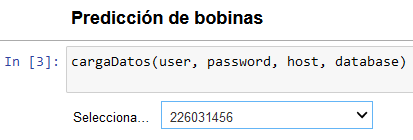
\includegraphics[width=0.7\textwidth]{img/celda3.PNG}
 \caption{Ejecución de la Tercera Celda}
 \label{f:celda3}
\end{figure}

También, en el directorio \texttt{./bobinas} se verán los diferentes CSV asociados a las bobinas sobre las que se han realizado predicciones. Además, junto al \emph{notebook} de la aplicación, se encontrará el fichero historia.txt donde se podrá consultar las predicciones de todas las bobinas.

Tras usar la aplicación, sería tan sencillo como cerrar la pestaña de la aplicación y finalmente cerrar la consola desde la que se ha lanzado \emph{Jupyter Notebook}, y de esta forma se detendría todo el proceso.